\chapter{Métricas de Software}
\label{chap:metricas}

\section{Processo de Medição}

A \citeonline{ISO:15939} define medição como a união de operações cujo objetivo é atribuir um valor a uma métrica. Ainda segundo a \citeonline{ISO:15939}, o processo de medição é a chave primária para a gerência de um software e suas atividades no seu ciclo de vida, além disso, um processo de melhoria contínua requer mudanças evolutivas e mudanças evolutivas requerem um processo de medição.
	Complementando o conceito levantado anteriormente, é possível afirmar de acordo com a \citeonline{ISO:9126} que a medição é a utilização de uma métrica para  atribuir um valor, que pode ser um número ou uma categoria, obtido a partir de uma escala a um atributo de uma entidade.
	A escala, citada anteriormente, pode ser definida como um conjunto de categorias para as quais os atributos estão mapeados, de modo que um atributo de medição está associado a uma escala \citeonline{ISO:15939}. Essas escalas podem ser divididas em:	

	\begin{easylist}[itemize]	
	
	& \textbf{Nominal:} A ordem não possui significado na interpretação dos valores \cite{Meirelles2013}
	& \textbf{Ordinal:} A ordem dos valores possui significado, porém a distância entre os valores não. \cite{Meirelles2013}
	& \textbf{Intervalo:}  A ordem dos valores possui significado e a distância entre os valores também. Porém, a proporção entre os valores não necessariamente possui significado. \cite{Meirelles2013}
	& \textbf{Racional:} Semelhante a a medida com escala do tipo intervalo, porém a proporção possui significado. \cite{Meirelles2013}

	\end{easylist}	
	
	A \citeonline{ISO:15939} divide o processo de medição em dois métodos diferentes, que se distinguem pela natureza do que é quantificado:
	
	\begin{easylist}[itemize]

	& \textbf{Subjetiva:} Quantificação envolvendo julgamento de um humano
	& \textbf{Objetiva:} Quantificação baseada em regras numéricas. Essas regras podem ser implementadas por um humano.

	\end{easylist}


%---------------------------------------------------------------------------------------------------------------------%

\section{Definição das métricas de software}

\citeonline{Fenton98}, mostraram que o termo métricas de software abrange muitas atividades, as quais estão envolvidas em um certo grau de medição de um software, como por exemplo estimativa de custo, estimativa de esforço e capacidade de reaproveitamento de elementos do software. Nesse contexto \citeonline{ISO:9126} categoriza as seguintes métricas de acordo com os diferentes tipos de medição:

\begin{easylist}[itemize]

 & \textbf{Métricas internas:} Aplicadas em um produto de software não executável, como código fonte. Oferecem aos usuários, desenvolvedores ou avaliadores o benefício de poder avaliar a qualidade do produto antes que ele seja executável.
& \textbf{Métricas externas:} Aplicadas a um produto de software executável, medindo o comportamento do sistema do qual o software é uma parte através de teste, operação ou mesmo obervação. Oferecem aos usuários, desenvolvedores ou avaliadores o benefício de poder avaliar a qualidade do produto durante seu processo de teste ou operação.
& \textbf{Métricas de qualidade em uso:} Aplicadas para medir o quanto um produto atende as necessidades de um usuário para que sejam atingidas metas especificadas como eficácia, produtividade, segurança e satisfação.

\end{easylist}

A figura abaixo reflete como as métricas influenciam nos contextos em que elas estão envolvidas, seja em relação ao software propriamente dito (tanto internamente quanto externamente) ou ao efeito produzido pelo uso de software:

	
\begin{figure}[h!]
\centering
\includegraphics[keepaspectratio=false,scale=0.90]{figuras/figuras_matheus/tipos_medidas_INGLES.eps}
\caption{Modelo de Qualidade do Produto da ISO 25023 adaptado da 
\citeonline{ISO25023}}
\label{modelodequalidade}
\end{figure}
\FloatBarrier

%---------------------------------------------------------------------------------------------------------------------%

\section{Métricas de código fonte}

Serão utilizadas nesse trabalho de conclusão de curso métricas de código fonte, que segundo \citeonline{Meirelles2013} são métricas do tipo objetiva calculadas a partir da análise estática do código fonte de um software. As métricas de código fonte serão divididas em duas categorias, seguindo a categorização adotada por \citeonline{rego_monitoramento_2014}: Métricas de tamanho e complexidade e métricas de orientação a objetos.

%--------------------------------------------
\subsection{Métricas de tamanho e complexidade}

O tamanho do código-fonte de um sistema foi um dos primeiros conceitos mensuráveis de software, uma vez que softwares podiam ocupar espaço tanto em forma de cartão perfurado quanto em forma de papel quando o código era impresso. Na programação em Assembler, por exemplo, uma linha física de código era o mesmo que uma instrução, logo, quanto maior o tamanho do código, maior era sua complexidade \cite{metricsandmodels}. A seguir são apresentadas algumas métricas de tamanho e complexidade.

\begin{easylist}[itemize]

	& \textbf{LOC} (\textit{Lines of Code}): Métrica simples em que são contadas as linhas executáveis de um código, desconsiderando linhas em branco e comentários.  \cite{metricsandmodels} 
		
	& \textbf{ACCM} (\textit{Average Cyclomatic Complexity per Method}): Mede a complexidade do programa, podendo ser representada através de um grafo de fluxo de controle. \cite{McCabe76}

	& \textbf{AMLOC} (\textit{Average Method Lines of Code}): Indica a distribuição de código entre os métodos. Quanto maior o valor da métrica, mais pesado é o método. É preferível que haja muitos métodos com pequenas operações do que um método grande e de entendimento complexo. \cite{Meirelles2013}
	
\end{easylist}

\subsection{Métricas de Orientação a Objetos}

O surgimento da programação orientada a objetos representou uma importante mudança na estratégia de desenvolvimento, focalizando a atenção para conceitos mais próximos ao negócio modelado. \cite{phpmysql}  

Métricas de orientação a objetos foram adotadas devido à grande utilização desse paradigma no desenvolvimento de software. Serão adotadas as seguintes métricas já selecionadas por \citeonline{rego_monitoramento_2014}:  

\begin{easylist}
	
	%--------------------------
	& \textbf{ACC} (\textit{Afferent Connections per Class} - Conexões Aferentes por Classe): Mede a conectividade entre as classes. Quanto maior a conectividade entre elas, maior o potencial de impacto que uma alteração pode gerar. \cite{Meirelles2013}
	
	%--------------------------
	& \textbf{ANPM} (\textit{Average Number of Parameters per Method} - Média do Número de Parâmetros por Método): Indica a média de parâmetros que os métodos possuem. Um valor muito alto para quantidade de parâmetros pode indicar que o método está tendo mais de uma responsabilidade. \cite{Basili1987}

	%--------------------------
	& \textbf{CBO} (\textit{Coupling Between Objects} - Acoplamento entre Objetos): Essa é uma métrica que diz respeito a quantas outras classes dependem de uma classe. É a conta das classes às quais uma classe está acoplada. 		Duas classes estão acopladas quando métodos de uma delas utilizam métodos ou variáveis de outra. Altos 			valores dessa métrica aumentam a complexidade e diminuem a manutenibilidade.  \cite{softwaremeasurementandestimation}.
  		 
	%-----------------------------
	& \textbf{DIT} (\textit{Depth of Inheritance Tree} - Profundidade da 
	Árvore de Herança): Responsável por medir quantas camadas de herança compõem uma determinada hierarquia 		de classes \cite{softwaremeasurementandestimation}. Segundo \citeonline{Meirelles2013}, quanto maior o valor de DIT, maior o número de métodos e atributos herdados, portanto maior a complexidade.

	%--------------------------
	& \textbf{LCOM4} (\textit{Lack of Cohesion in Methods} - Falta de Coesão
	entre Métodos): A coesão de uma classe é indicada por quão próximas as variáveis locais estão relacionadas com variáveis de instância locais. Alta coesão indica uma boa subdivisão de classes. A LCOM mede a falta de coesão através dissimilaridade dos métodos de uma classe pelo emprego de variáveis de instância.\cite{metricsandmodels}. A métrica LCOM foi revista e passou a ser conhecida como LCOM4, sendo necessário para seu cálculo a construção de um gráfico não-orientado em que os nós são os atributos e métodos de uma classe. Para cada método deve haver uma aresta entre ele e outro método ou variável. O valor da LCOM4 é o número de componentes fracamente conectados a esse gráfico \cite{Meirelles2013}

	%--------------------------
	& \textbf{NOC} (\textit{Number of Children} - Número de Filhos): É o número de sucessores imediatos,  (portanto filhos) de uma classe. Segundo \citeonline{softwaremeasurementandestimation}, altos valores indicam que a abstração da super classe foi diluída e uma reorganização da arquitetura deve ser considerada.
	
	%-----------------------------
	& \textbf{NOM} (\textit{Number of Methods} - Número de Métodos): Indica a quantidade de métodos de uma classe, medindo seu tamanho. Classes com muitos métodos são mais difíceis de serem reutilizadas pois são propensas a serem menos coesas. \cite{Meirelles2013}  

	%-----------------------------
	& \textbf{NPA} (\textit{Number of Public Attributes} - Número de Atributos Públicos): Mede o encapsulamento de uma classe, através da medição dos atributos públicos. O número ideal para essa métrica é zero \cite{Meirelles2013}

	%-----------------------------
	& \textbf{RFC} (\textit{Response For a Class} - Respostas para uma Classe): \citeonline{metricsandmodels} define essa métrica como o número de métodos que podem ser executados em respostas a uma mensagem recebida por um objeto da classe.

\end{easylist}	

%---------------------------------------------------------------------------------------------------------------------%

\section{Configurações de qualidade para métricas de código fonte} 

Em sua tese de doutorado, \citeonline{Meirelles2013} buscou responder as seguintes questões de pesquisa:
\begin{easylist}[itemize]

	& \textbf{QP1 -} Métricas de código-fonte podem influir na atratividade de projetos de software livre? 
	& \textbf{QP1 -} Quais métricas devem ser controladas ao longo do tempo?		
	& \textbf{QP3 -} As métricas de código-fonte melhoram com o amadurecimento do projeto?	
	
\end{easylist}

Para responder essas questões, sua pesquisa concentrou-se em alguns objetivos tecnológicos e científicos, fazendo uso da técnica estatística descritiva percentil para identificação das distribuições dos valores de métricas em 38 projetos de software livre, observando os valores frequentes dessas métricas de modo a servirem de referência para projetos futuros. 

O percentil são pontos estimativos de uma distribuição de frequência que determinam a porcentagem de elementos que se encontram abaixo deles. Por exemplo, quando se diz que o valor 59,0 da métrica rfc do projeto \textbf{Open JDK8} está no percentil 90, significa dizer que 90\% dos valores identificados para essa métrica estão abaixo de 59,0. 

A tabela \ref{tab:percentil} abaixo pôde ser criada graças ao uso da técnica estatística citada:
	
	\begin{table}[!ht]
	\begin{center}
	
	\input{tabelas/tabelasMatheus/percentis.ltx} 
	\caption{Percentis para métrica RFC em projetos Java extraídos de  
	\citeonline{Meirelles2013}}
	\label{tab:percentil}
	\end{center}
	\end{table}	
	\FloatBarrier	

Através dos resultados obtidos para cada métrica, \citeonline{Meirelles2013} observou que era possível identificar valores frequentes analisando os percentis. Na \ref{tab:percentil}, por exemplo, foram observados no projeto \textbf{Open JDK8} valores de 0 a 9 como muito frequentes, de 10 a 26 como frequente, de 27 a 59 como pouco frequente e acima de 59, que representa apenas 10\% do código-fonte do projeto, como não frequente \cite{Meirelles2013}. A seguinte tabela foi extraída do trabalho de conclusão de curso de \citeonline{rego_monitoramento_2014} para que fosse criada uma relação entre o intervalo de frequência e o intervalo qualitativo de uma métrica, afim de facilitar sua interpretação:

\begin{table}[!ht]
	\begin{center}
	\input{tabelas/tabelasMatheus/intervalos.ltx}
	\caption{Nome dos Intervalos de Frequência extraídos de \citeonline{rego_monitoramento_2014}}
	\label{tab:nomes}
	\end{center}
	\end{table}
	\FloatBarrier
	
	 
\citeonline{Meirelles2013} destaca na avaliação dos resultados a maneira como o \textbf{Open JDK8} demonstrou um equilíbrio no valor das métricas em relação aos demais projetos Java, de modo que seus valores são frequentemente usados como referência na interpretação dos valores das métricas. Se de um lado o  \textbf{Open JDK8} demonstrou os menores valores percentis, os valores mais altos foram identificados no \textbf{Tomcat}. \citeonline{rego_monitoramento_2014} considerou então os dois cenários para que as referências de valores para as métricas fossem criadas. O resultado dessa análise gerou em seu trabalho a seguinte tabela:

\begin{table}[!ht]
	\begin{center}
	\input{tabelas/tabelasMatheus/metricas.ltx}	
	\caption{Configurações para os Intervalos das Métricas para Java extraídas de \citeonline{rego_monitoramento_2014}}
	\label{tab:good-metrics}
	\end{center}
	\end{table}
	\FloatBarrier
   

%---------------------------------------------------------------------------------------------------------------------%

\section{Cenários de limpeza} 

Em seu livro Implementation Patterns, \citeonline{Beck2007} destaca três valores que um código limpo precisa ter: Comunicabilidade , simplicidade e flexibilidade.
	
\begin{easylist}[itemize]

	& \textbf{Comunicabilidade:} Um código se expressa bem quando alguém que o lê é capaz de compreendê-lo e modificá-lo. \citeonline{Beck2007} destaca que quando foi necessário modificar um código, ele gastou muito mais tempo lendo o que já havia sido feito do que escrevendo sua modificação 
		
	& \textbf{Simplicidade:} Eliminar o excesso de complexidade faz com que aqueles que estejam lendo o código a entendê-lo mais rapidamente. O excesso de complexidade faz com que seja maior a probabilidade de erro e com que seja mais difícil fazer uma manutenção no futuro.Buscar simplicidade é também buscar inovação: \textit{Junit} é muito mais simples que muitas ferramentas de teste que ele substituiu.

	& \textbf{Flexibilidade:} Capacidade de estender a aplicação alterando o mínimo possível a estrutura já criada.
		
\end{easylist}	

Buscando levantar conceitos que fizessem com que um código atendesse os valores citados acima, tornando-se assim um código limpo, \citeonline{almeida_codigo} levantaram em seu trabalho conceitos de limpeza, evidenciando as contribuições e consequências que o uso da técnica pode causar no código. Serão citadas a seguir técnicas levantadas por \citeonline{almeida_codigo} que ganharam destaque no trabalho de \citeonline{rego_monitoramento_2014}:

 \begin{table}[!ht]
\centering
\input{tabelas/tabelasMatheus/conceitos-limpeza.ltx}
\caption{Conceitos de Limpeza levantados por \citeonline{almeida_codigo} extraídos de \citeonline{rego_monitoramento_2014}}
\label{tab:conceitos}
\end{table}
\FloatBarrier

Após o levantamento dos conceitos de limpeza, \citeonline{almeida_codigo} criaram um mapeamento os relacionando com métricas de código, definindo cenários de limpeza. O objetivo, como ressaltado pelo autor, não era classificar um código como limpo ou não, mas sim facilitar melhorias de implementação através da aproximação dos valores das métricas com os esperados nos contextos de interpretação.

Aproveitando inicialmente os cenários \textbf{Classe pouco coesa} e \textbf{Interface dos métodos} extraídos de  \citeonline{almeida_codigo}, \citeonline{rego_monitoramento_2014} elaborou mais alguns cenários de limpeza, utilizando como referência a configuracão do \textbf{Open JDK8}, considerando como valores altos os valores obtidos pelos intervalos  Regular e Ruim para esse sistema. O resultado dessa atividade pode ser vista na tabela abaixo:

\begin{sidewaystable}
\begin{table}[H]
\centering
\input{tabelas/tabelasMatheus/cenarios.ltx}
\caption{Cenários de Limpeza extraídos de \citeonline{rego_monitoramento_2014}}
\label{tab:cenarios}
\end{table}
\FloatBarrier
\end{sidewaystable}  

  